\documentclass[11pt]{article}

\usepackage[a4paper,margin=23mm]{geometry}
\usepackage[T1]{fontenc}
\usepackage[utf8]{inputenc}
\usepackage{amsmath,amssymb}
\usepackage{array}
\usepackage{booktabs}
\usepackage{enumitem}
\usepackage{longtable}
\usepackage{tabularx}
\usepackage{xcolor}
\usepackage{listings}
\usepackage{tikz}
\usetikzlibrary{arrows.meta,calc,fit,positioning,shapes.geometric}
\usepackage[hidelinks]{hyperref}

\setlength{\parindent}{0pt}
\setlength{\parskip}{0.55em}
\setlist{leftmargin=*,nosep}
\emergencystretch=3em
\renewcommand{\arraystretch}{1.16}
\setcounter{tocdepth}{2}

\definecolor{codebg}{RGB}{247,247,247}
\definecolor{rulegrey}{RGB}{92,92,92}
\definecolor{causalblue}{RGB}{31,78,121}
\definecolor{evidencegreen}{RGB}{46,125,50}
\definecolor{warningred}{RGB}{176,48,48}
\definecolor{softblue}{RGB}{232,241,249}
\definecolor{softgreen}{RGB}{235,246,235}
\definecolor{softred}{RGB}{252,237,237}
\definecolor{softgrey}{RGB}{242,242,242}

\lstset{
  basicstyle=\ttfamily\small,
  backgroundcolor=\color{codebg},
  frame=single,
  rulecolor=\color{rulegrey},
  breaklines=true,
  columns=fullflexible,
  keepspaces=true,
  showstringspaces=false,
  aboveskip=0.7em,
  belowskip=0.7em
}

\tikzset{
  var/.style={circle,draw=causalblue,very thick,fill=softblue,
    minimum size=9mm,inner sep=1pt,font=\bfseries},
  irrelevant/.style={circle,draw=warningred,very thick,dashed,fill=softred,
    minimum size=9mm,inner sep=1pt,font=\bfseries},
  flow/.style={-{Latex[length=2.4mm]},very thick,draw=causalblue},
  process/.style={draw=causalblue,rounded corners,thick,fill=softblue,
    align=center,inner sep=6pt},
  evidencebox/.style={draw=evidencegreen,rounded corners,thick,fill=softgreen,
    align=center,inner sep=6pt},
  warningbox/.style={draw=warningred,rounded corners,thick,fill=softred,
    align=center,inner sep=6pt},
  neutralbox/.style={draw=rulegrey,rounded corners,thick,fill=softgrey,
    align=center,inner sep=6pt},
  smalllabel/.style={font=\small,align=center}
}

\DeclareRobustCommand{\code}[1]{\texttt{\detokenize{#1}}}
\newcommand{\ABALearn}{\textsc{ABALearn}}
\newcommand{\Hprobe}[1]{\textbf{H#1}}
\newcommand{\Epos}{E^{+}}
\newcommand{\Eneg}{E^{-}}
\newcommand{\indep}{\perp\!\!\!\perp}
\newcommand{\notindep}{\not\!\perp\!\!\!\perp}
\newcommand{\question}{\paragraph{Question and purpose.}}
\newcommand{\comparison}{\paragraph{Controlled comparison.}}
\newcommand{\observation}{\paragraph{Emphasised observation.}}
\newcommand{\explanation}{\paragraph{Trace-supported explanation.}}
\newcommand{\boundary}{\paragraph{Evidential boundary.}}
\newcommand{\record}[1]{\par\smallskip\noindent\textit{Primary evidence record: }
  \path{#1}\par}

\title{What Target-wise ABA Learning Does on\\
Deterministic Causal Fixtures\\[0.35em]
\large Evidence from M1.3 Bucket 3, H0--H7b}
\author{Working synthesis for discussion with Fabrizio}
\date{4 August 2026}

\begin{document}
\maketitle

\begin{center}
\fbox{\begin{minipage}{0.93\textwidth}
\textbf{Status and purpose.}
This is a supervisor-facing working document. It introduces the causal
fixture, learner input, terminology, configurations, and experimental sequence
before stating any cross-cutting findings. H0--H7b are complete and analysed,
but Bucket~3 still has no approved claim. The six Findings headings and the
Implications heading at the end are intentionally empty placeholders for
subsequent drafting and review.
\end{minipage}}
\end{center}

\begin{abstract}
The investigation asks what target-wise ABA Learning does when given only a
finite binary table sampled from a known causal data-generating process. The
principal process has independent stochastic roots and a deterministic AND
child. The graph, mechanisms, population distribution, finite sample,
learner-visible encoding, learned ABA framework, and evaluator-only reference
are kept separate throughout.

The experimental sequence begins with a baseline comparison across targets and
then introduces one controlled question at a time: sample support, irrelevant
variables, background-knowledge order, brave versus cautious learning,
folding-token budget, grounded sample size, and the \code{relto} versus
\code{sechk} assumption-introduction options. This document records what each
probe was intended to reveal, its principal signal, and the procedural
explanation supported by the generated deltas and Prolog traces. It does not
describe the current pipeline as full Causal ABA or full causal discovery.
\end{abstract}

\tableofcontents
\newpage

\section{Purpose, scope, and organising question}

\subsection{Research question}

\begin{quote}
Given a finite table sampled from a known deterministic causal fixture, what
rules and ABA structures does target-wise \ABALearn{} produce; under which
conditions do those structures correspond to the generating mechanism; and
what explains the departures from it?
\end{quote}

The purpose is not merely to count procedural solutions. It is to describe
how the learner transforms the supplied table into rules, assumptions, and
contraries, and to distinguish several possible outcomes:

\begin{itemize}
  \item recovery of a rule that coincides with the deterministic mechanism;
  \item a sample-adequate but non-minimal rule;
  \item a defeasible representation that differs from the mechanism;
  \item a rule supported only because a population counterexample is absent
  from the finite sample;
  \item an assumption construction that satisfies the selected learning
  semantics without defining the target from its predictors; and
  \item failure or timeout caused by the configured search procedure.
\end{itemize}

These distinctions are necessary before asking whether learned target-wise
theories can contribute to causal graph discovery. A predictive or
sample-covering rule is not automatically causal, and a successful learner
exit status is not automatically a mechanism-recovery result.

\subsection{Scope}

The evidence concerns three small binary fixtures, fixed seed-42 samples, and
the repository configurations described below. The investigation is
target-wise: for a fixed table, each observed variable is used as the target
in a separate learning run. Changing the target changes the examples and BK
encoding, but does not create a new sample.

The deterministic child \(C\) is the only variable with a desirable
deterministic rule over its observed parents. Root-target runs are nevertheless
essential diagnostics. They test whether the learner refuses to invent a
deterministic relationship where the data-generating process supplies none,
and they expose the effects of finite support, learning semantics, and search
budget.

\subsection{Relation to Causal ABA}

The current pipeline is target-wise ABA Learning over encoded tabular data.
It learns rules, assumptions, and contraries from BK and labelled examples.
It does not yet implement the Russo-style Causal ABA machinery in which
assumptions directly encode arrows, no-edge statements, or conditional
independences, graph-theoretic constraints encode acyclicity and
\(d\)-separation, and stable extensions correspond to compatible candidate
DAGs.

Consequently, the present evidence concerns learned rule structure and learner
behaviour. It is groundwork for deciding how causal or probabilistic
information might later guide, constrain, or interpret ABA Learning. It does
not itself output a DAG, MEC, or CPDAG.

\section{Conceptual framework and notation}

\subsection{The seven objects that must not be conflated}

The experimental reasoning separates the following objects:

\begin{enumerate}
  \item a generating DAG \(G\);
  \item structural mechanisms for the variables in \(G\);
  \item the exact observational population distribution \(P^\ast\);
  \item a finite IID sample \(\mathcal{D}_n\sim P^\ast\);
  \item target-specific learner input derived from \(\mathcal{D}_n\);
  \item the learned ABA framework and its emitted delta; and
  \item evaluator-side judgements about sample adequacy, mechanism alignment,
  minimality, and causal meaning.
\end{enumerate}

\begin{figure}[ht]
\centering
\resizebox{0.97\textwidth}{!}{%
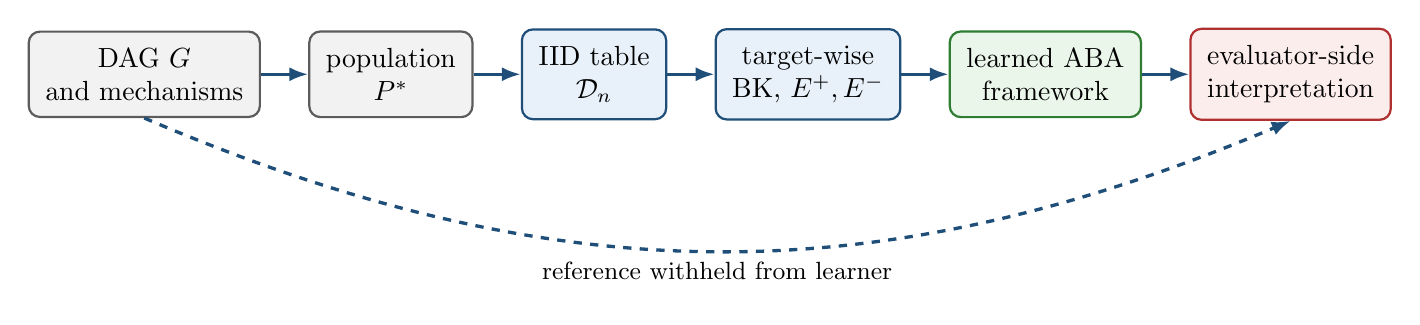
\begin{tikzpicture}[node distance=6mm]
  \node[neutralbox] (dag) {DAG \(G\)\\and mechanisms};
  \node[neutralbox,right=of dag] (pop) {population\\\(P^\ast\)};
  \node[process,right=of pop] (sample) {IID table\\\(\mathcal{D}_n\)};
  \node[process,right=of sample] (encode) {target-wise\\BK, \(\Epos,\Eneg\)};
  \node[evidencebox,right=of encode] (learn) {learned ABA\\framework};
  \node[warningbox,right=of learn] (eval) {evaluator-side\\interpretation};
  \draw[flow] (dag) -- (pop);
  \draw[flow] (pop) -- (sample);
  \draw[flow] (sample) -- (encode);
  \draw[flow] (encode) -- (learn);
  \draw[flow] (learn) -- (eval);
  \draw[flow,dashed] (dag.south) to[bend right=23]
    node[below,smalllabel] {reference withheld from learner} (eval.south);
\end{tikzpicture}
}
\caption{Experimental separation. Only the finite table and its target-wise
encoding cross the learner boundary. The generating graph and mechanism
reference are used only for evaluation.}
\label{fig:object-separation}
\end{figure}

These levels answer different questions. Faithfulness is a property of
\(P^\ast\) relative to \(G\), not of one finite table. A learned implication
may hold on \(\mathcal{D}_n\) but fail in \(P^\ast\). A learned rule may mention
a parent without establishing the direction of a causal edge.

\subsection{ABA framework}

An ABA framework is a tuple
\[
\mathcal{F}=\langle\mathcal{L},\mathcal{R},\mathcal{A},
\overline{\cdot}\rangle,
\]
where \(\mathcal{L}\) is a language, \(\mathcal{R}\) is a set of rules,
\(\mathcal{A}\subseteq\mathcal{L}\) is a set of assumptions, and
\(\overline{\cdot}\) maps each assumption to its contrary.

A rule has the form
\[
h\leftarrow b_1,\ldots,b_m.
\]
If \(m=0\), it is a fact. Assumptions are defeasible premises: an argument may
use an assumption \(\alpha\), but deriving \(\overline{\alpha}\) attacks it.
A stable extension is, informally, a coherent set of accepted assumptions
which attacks every assumption outside it. The learned framework can therefore
represent an ordinary rule together with explicit exceptional conditions.

\subsection{ABA Learning task}

An ABA Learning task begins with background knowledge and two finite sets of
examples:
\[
\Epos=\{e^+_1,\ldots,e^+_p\},\qquad
\Eneg=\{e^-_1,\ldots,e^-_q\}.
\]
The learner applies symbolic transformations to construct a framework
\(\mathcal{F}'\) under which the examples satisfy the selected consequence
condition. The learned object is an ABA framework, not a fitted numerical
parameter vector.

The transformations relevant here are:

\begin{itemize}
  \item \textbf{Rote learning.} Add example-specific rules from the positive examples.
  \item \textbf{Folding.} Replace example-specific conditions with reusable BK
  predicates, producing intensional rules.
  \item \textbf{Subsumption.} Remove a specialised rule when an appropriate more
  general rule already exists.
  \item \textbf{Assumption introduction.} Make an over-general rule defeasible by
  adding an assumption; learn rules for its contrary to represent exceptions.
\end{itemize}

\subsection{Exact-value target-wise encoding}

For each row identifier \(i\), every non-target variable is represented by
exactly one value predicate. When \(c\) is the target, for example, the BK
contains facts such as

\begin{lstlisting}
a_val_1(9).
b_val_0(9).
\end{lstlisting}

and row 9 contributes either \(c(9)\in\Epos\) or \(c(9)\in\Eneg\), according to
its target value. For a binary target \(Y\),
\[
\Epos_Y=\{Y(i):Y_i=1\},\qquad
\Eneg_Y=\{Y(i):Y_i=0\}.
\]
All non-target columns are available as BK predictors in their serialized
order. This creates a symmetric target interface, but it does not make the
variables causally symmetric: a deterministic child and a stochastic root
have different evaluator-side recovery objects.

\begin{figure}[ht]
\centering
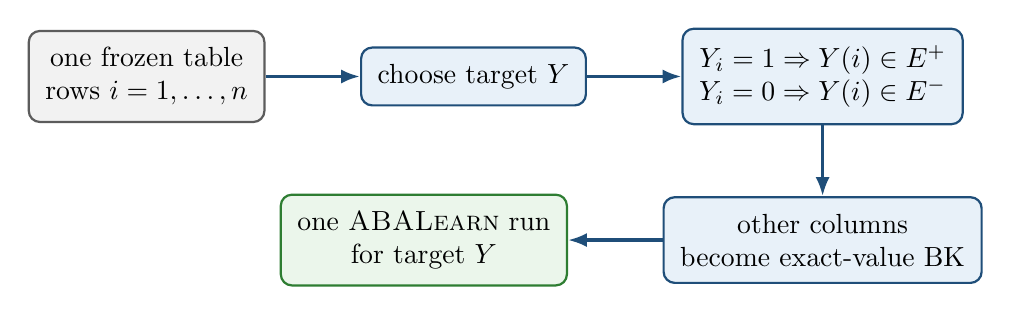
\begin{tikzpicture}[node distance=9mm and 12mm]
  \node[neutralbox] (table) {one frozen table\\rows \(i=1,\ldots,n\)};
  \node[process,right=of table] (target) {choose target \(Y\)};
  \node[process,right=of target] (examples)
    {\(Y_i=1\Rightarrow Y(i)\in\Epos\)\\
     \(Y_i=0\Rightarrow Y(i)\in\Eneg\)};
  \node[process,below=of examples] (bk)
    {other columns\\become exact-value BK};
  \node[evidencebox,left=of bk] (run)
    {one \ABALearn{} run\\for target \(Y\)};
  \draw[flow] (table) -- (target);
  \draw[flow] (target) -- (examples);
  \draw[flow] (examples) -- (bk);
  \draw[flow] (bk) -- (run);
\end{tikzpicture}
\caption{Target-wise encoding. All targets use the same rows; the selected
target determines the positive and negative examples and the remaining
columns determine the BK.}
\label{fig:targetwise-encoding}
\end{figure}

\subsection{Brave and cautious learning}

Let \(\operatorname{Stab}(\mathcal{F}')\) be the stable extensions of the
learned framework. Brave learning uses an existential witness: there must be
some \(\Delta\in\operatorname{Stab}(\mathcal{F}')\) which simultaneously
accepts every positive example and rejects every negative example. In compact
form,
\[
\exists\Delta\in\operatorname{Stab}(\mathcal{F}')
\quad
\bigl[
  \forall e\in\Epos,\ \mathcal{F}'\models_\Delta e
  \ \land\
  \forall e\in\Eneg,\ \mathcal{F}'\not\models_\Delta e
\bigr].
\]

Cautious acceptance requires a claim to be accepted with respect to every
stable extension. A cautious learning solution therefore requires all
positives to be cautious consequences and requires each negative not to be a
cautious consequence:
\[
\forall e\in\Epos,\ \mathcal{F}'\models_{\mathrm{caut}}e,
\qquad
\forall e\in\Eneg,\ \mathcal{F}'\not\models_{\mathrm{caut}}e.
\]

This distinction matters whenever introduced assumptions permit more than one
stable extension. Brave learning may use one joint witnessing extension.
Cautious learning tests whether a positive survives every stable extension.
Neither mode by itself establishes that a target is a deterministic function
of the supplied predictors.

\subsection{Greedy and non-deterministic folding}

The configurations studied here use two different search strategies.

\paragraph{Greedy folding.}
The AAMAS configuration greedily folds a rote rule over the matching
exact-value BK literals, with \code{mgr} selection and BK folding space. In the
current complete exact-value representation, its solved Horn rules can become
maximal co-occurrence descriptions. Folding is applied per rule; the learner
does not subsequently synthesise a more general rule by deleting a literal
across several complementary rules.

\paragraph{Non-deterministic folding.}
The nd configurations fold incrementally with \code{any} selection and the
larger \code{all} folding space. A first admissible BK predicate can therefore
become the first generalising fold. If that rule over-generalises, assumption
introduction and contrary learning can preserve the initial fold while adding
defeasible repair structure around it.

Greedy and nd configurations change a bundle of settings. A direct
AAMAS-versus-ECAI comparison can reveal different behaviour, but it cannot
attribute that difference to folding mode alone.

\subsection{The \code{relto} and \code{sechk} assumption-introduction options}

Both options are invoked when a folded candidate fails the relevant
entailment check and the learner attempts to make the rule defeasible. They
choose different procedural routes.

\paragraph{\code{asm_intro(relto)}.}
The learner first searches for an assumption relative to the current folded
body. In the inspected traces, a failed reuse can return KO and permit
backtracking to a different folding literal. This is how later BK variables
can enter contrary rules.

\paragraph{\code{asm_intro(sechk)}.}
The learner first generates a new provisional assumption and tests the
resulting framework through the \code{gen5}/\code{gen6} semantic-checking
path. Depending on the learning semantics, the provisional assumption may
close a repair early or may itself be rejected, forcing further nesting and
search.

\begin{figure}[ht]
\centering
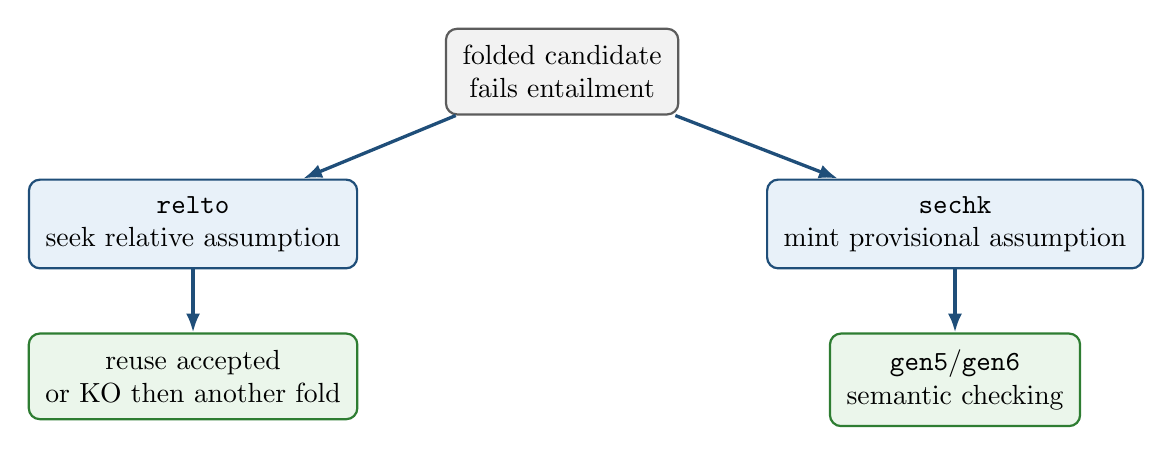
\begin{tikzpicture}[node distance=8mm and 11mm]
  \node[neutralbox] (failed) {folded candidate\\fails entailment};
  \node[process,below left=of failed] (relto)
    {\code{relto}\\seek relative assumption};
  \node[process,below right=of failed] (sechk)
    {\code{sechk}\\mint provisional assumption};
  \node[evidencebox,below=of relto] (reuse)
    {reuse accepted\\or KO then another fold};
  \node[evidencebox,below=of sechk] (semantic)
    {\code{gen5}/\code{gen6}\\semantic checking};
  \draw[flow] (failed) -- (relto);
  \draw[flow] (failed) -- (sechk);
  \draw[flow] (relto) -- (reuse);
  \draw[flow] (sechk) -- (semantic);
\end{tikzpicture}
\caption{Repository assumption-introduction fork. H7 changes only this option
within a fixed brave-nd or cautious-nd bundle. The subsequent path is also
conditioned by the selected entailment semantics.}
\label{fig:assumption-introduction}
\end{figure}

\code{relto} and \code{sechk} are implementation options, not causal
criteria. A variable reached by one path is not thereby causal, and a shorter
or longer learned theory is not automatically more correct.

\subsection{Evaluation vocabulary}

\begin{center}
\small
\begin{tabularx}{\textwidth}{
  >{\raggedright\arraybackslash}p{0.25\textwidth}X}
\toprule
Term & Meaning in this document \\
\midrule
\code{solved} & The learner emitted an accepted framework under the selected
configuration and semantics. \\
\code{completed_no_solution} & Search terminated without an accepted theory,
relative to the configured strategy and resource ceiling. \\
\code{timeout} & The wall-time limit was reached; this is not evidence of
unlearnability. \\
Sample-adequate & The framework satisfies the encoded finite examples under
the chosen semantics. \\
Mechanism-aligned string & A learned rule is syntactically identical to the
evaluator-only deterministic rule. \\
Distractor-retaining & A learned theory refers to a variable absent from the
target mechanism. \\
Spurious finite-sample rule & A rule holds on the observed table but is false
in the generating population. \\
Mechanism recovery & A justified conclusion that the learned theory represents
the deterministic structural mechanism; stronger than \code{solved}. \\
Graph recovery & A justified conclusion about edges, orientations, an MEC, or
a CPDAG; not produced automatically by any target-wise delta. \\
\bottomrule
\end{tabularx}
\end{center}

The generated \code{bk.sol_chk.asp} file is an integrity-check artefact for the
serialized solution. Its satisfiability is not an independent graph-recovery
metric and, under cautious learning, is not by itself proof that every
positive is a cautious consequence.

\section{Causal fixtures and evaluator ground truth}

\subsection{H0 baseline: binary AND collider}

The principal fixture is
\[
G_0:\qquad A\longrightarrow C\longleftarrow B,
\]
with learner identifiers \(a,b,c\). The roots are mutually independent:
\[
A\sim\operatorname{Bernoulli}(4/5),
\qquad
B\sim\operatorname{Bernoulli}(7/10),
\qquad
A\indep B.
\]
The child is deterministic:
\[
C=A\land B.
\]

\begin{figure}[ht]
\centering
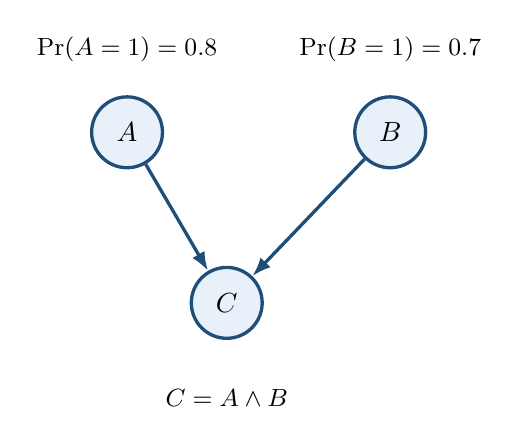
\begin{tikzpicture}[node distance=15mm and 24mm]
  \node[var] (a) {$A$};
  \node[var,right=of a] (b) {$B$};
  \node[var,below right=15mm and 6mm of a] (c) {$C$};
  \draw[flow] (a) -- (c);
  \draw[flow] (b) -- (c);
  \node[smalllabel,above=3mm of a] {\(\Pr(A=1)=0.8\)};
  \node[smalllabel,above=3mm of b] {\(\Pr(B=1)=0.7\)};
  \node[smalllabel,below=5mm of c] {\(C=A\land B\)};
\end{tikzpicture}
\caption{H0 generating DAG. Randomness enters through the independent roots;
the non-root mechanism is deterministic.}
\label{fig:h0-dag}
\end{figure}

The induced population distribution is:

\begin{center}
\begin{tabular}{@{}cccc@{}}
\toprule
\(A\) & \(B\) & \(C\) & \(P^\ast(A,B,C)\) \\
\midrule
0 & 0 & 0 & \(3/50=0.06\) \\
0 & 1 & 0 & \(7/50=0.14\) \\
1 & 0 & 0 & \(6/25=0.24\) \\
1 & 1 & 1 & \(14/25=0.56\) \\
\bottomrule
\end{tabular}
\end{center}

The remaining four binary assignments are structural zeros. Causal
sufficiency is supplied by the fixture design: the root exogenous noise terms
are mutually independent and there is no omitted common cause. The causal
Markov condition follows from
\[
P^\ast(a,b,c)=P^\ast(a)P^\ast(b)P^\ast(c\mid a,b).
\]
Ordinary faithfulness was verified exactly by auditing every singleton-pair
conditional-independence query against \(d\)-separation. The sole population
independence is \(A\indep B\); conditioning on the collider makes
\(A\notindep B\mid C\), and each parent is dependent on \(C\).

The skeleton is \(A-C-B\) and the unshielded collider is
\(A\rightarrow C\leftarrow B\). Consequently, the ordinary
conditional-independence MEC contains only this DAG and the CPDAG has both
arrows directed into \(C\). This population-level causal reference is never
shown to \ABALearn{}.

\subsection{Evaluator-only mechanism reference}

For H0, the canonical rule corresponding to the deterministic child mechanism
is:

\begin{lstlisting}
c(A) :- a_val_1(A), b_val_1(A).
\end{lstlisting}

Targets \(a\) and \(b\) are stochastic roots. Their evaluator reference is
\path{no_observed_parent_deterministic_rule}; there is no desired rule that
deterministically derives either root from the other observed variables.

Syntactic equality with the rule above is strong fixture-specific evidence,
but not sufficient on its own for graph recovery. Conversely, a different ABA
representation may be extensionally adequate without matching the canonical
string. The records therefore inspect rule structure, assumptions, contraries,
and the target's generating role separately.

\subsection{Frozen H0 sample}

The principal table is the seed-42 IID sample with \(n=30\):

\begin{center}
\begin{tabular}{@{}lr@{}}
\toprule
Assignment & Count \\
\midrule
\((1,1,1)\) & 17 \\
\((1,0,0)\) & 7 \\
\((0,1,0)\) & 4 \\
\((0,0,0)\) & 2 \\
\bottomrule
\end{tabular}
\end{center}

All four population atoms appear. The target example counts are
\[
a:24^+/6^-,
\qquad
b:21^+/9^-,
\qquad
c:17^+/13^-.
\]

For child \(c\), all positive examples have \(A=B=1\). For root target \(a\),
the predictor cell \((B,C)=(0,0)\) contains both target labels. In particular:

\begin{center}
\begin{tabular}{@{}ccccc@{}}
\toprule
Row & \(A\) target & \(B\) predictor & \(C\) predictor & Class for target \(a\) \\
\midrule
9 & 1 & 0 & 0 & positive \\
26 & 0 & 0 & 0 & negative \\
\bottomrule
\end{tabular}
\end{center}

No deterministic rule over \((B,C)\) can distinguish these two rows. Target
\(b\) has the symmetric ambiguity. This pair later provides the clearest test
of brave versus cautious assumption use.

\subsection{H2 and H3 controlled extensions}

\begin{figure}[ht]
\centering
\begin{minipage}[t]{0.47\textwidth}
\centering
\textbf{H2: trailing isolated \(D\)}

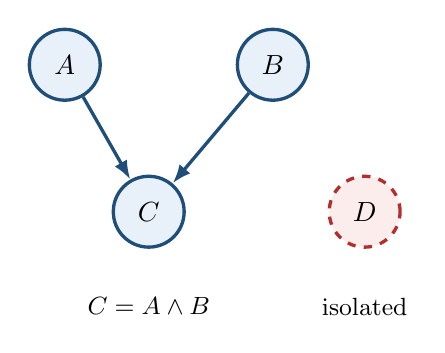
\begin{tikzpicture}[node distance=12mm and 17mm]
  \node[var] (a) {$A$};
  \node[var,right=of a] (b) {$B$};
  \node[var,below right=12mm and 4mm of a] (c) {$C$};
  \node[irrelevant,right=18mm of c] (d) {$D$};
  \draw[flow] (a) -- (c);
  \draw[flow] (b) -- (c);
  \node[smalllabel,below=5mm of c] {\(C=A\land B\)};
  \node[smalllabel,below=5mm of d] {isolated};
\end{tikzpicture}

\small target-\(c\) BK order: \([a,b,d]\)
\end{minipage}
\hfill
\begin{minipage}[t]{0.47\textwidth}
\centering
\textbf{H3: leading isolated \(A\)}

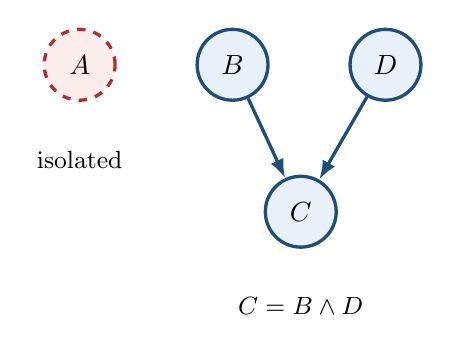
\begin{tikzpicture}[node distance=12mm and 15mm]
  \node[irrelevant] (a) {$A$};
  \node[var,right=10mm of a] (b) {$B$};
  \node[var,right=10mm of b] (d) {$D$};
  \node[var,below right=12mm and 2mm of b] (c) {$C$};
  \draw[flow] (b) -- (c);
  \draw[flow] (d) -- (c);
  \node[smalllabel,below=5mm of c] {\(C=B\land D\)};
  \node[smalllabel,below=5mm of a] {isolated};
\end{tikzpicture}

\small target-\(c\) BK order: \([a,b,d]\)
\end{minipage}
\caption{Controlled extensions. Dashed red nodes are independent isolated
variables. H2 appends the distractor after the mechanism parents; H3 places it
before them.}
\label{fig:extended-fixtures}
\end{figure}

H2 preserves the H0 collider and AND mechanism and adds an isolated
\(D\sim\operatorname{Bernoulli}(1/2)\). Its evaluator rule remains:

\begin{lstlisting}
c(A) :- a_val_1(A), b_val_1(A).
\end{lstlisting}

H3 instead uses independent roots
\[
A\sim\operatorname{Bernoulli}(1/2),\qquad
B\sim\operatorname{Bernoulli}(4/5),\qquad
D\sim\operatorname{Bernoulli}(7/10),
\]
with \(A\) isolated and \(C=B\land D\). Its evaluator rule is:

\begin{lstlisting}
c(A) :- b_val_1(A), d_val_1(A).
\end{lstlisting}

Both extensions have verified Markov factorisation and exact ordinary
faithfulness certificates. The evaluator graph and rules remain hidden from
the learner.

\section{Experimental design and comparison logic}

\subsection{Learner configurations}

\begin{center}
\small
\begin{tabularx}{\textwidth}{
  >{\raggedright\arraybackslash}p{0.21\textwidth}
  >{\raggedright\arraybackslash}p{0.10\textwidth}
  >{\raggedright\arraybackslash}p{0.13\textwidth}
  >{\raggedright\arraybackslash}p{0.12\textwidth}
  >{\raggedright\arraybackslash}p{0.12\textwidth}X}
\toprule
Identity & Semantics & Folding & Selection & Space & Assumption introduction \\
\midrule
\code{aamas2025} & brave & greedy & mgr & BK & \code{relto} \\
\code{ecai2024} & brave & nd & any & all & \code{relto} \\
\code{baseline_cautious} & cautious & nd & any & all & \code{relto} \\
\code{greedy_cautious} & cautious & greedy & mgr & BK & \code{relto} \\
\code{nd_brave_sechk} & brave & nd & any & all & \code{sechk} \\
\code{nd_cautious_sechk} & cautious & nd & any & all & \code{sechk} \\
\bottomrule
\end{tabularx}
\end{center}

\code{aamas2025} and \code{ecai2024} reproduce the relevant repository
configurations associated with the corresponding published approaches.
\code{baseline_cautious}, \code{greedy_cautious},
\code{nd_brave_sechk}, and \code{nd_cautious_sechk} are experimental
identities used for controlled comparison. In particular,
\code{greedy_cautious} is not a published \emph{AAMAS cautious} method.

The H6 configurations match \code{baseline_cautious} except for
\code{folding_steps}. H7a matches \code{ecai2024} except for
\code{asm_intro}; H7b matches \code{baseline_cautious} except for
\code{asm_intro}.

\subsection{Strength of comparisons}

Three levels of evidence are distinguished.

\begin{itemize}
  \item \textbf{Exact paired option ablation.} Fixture, sample, encoding, and all
  relevant learner settings are fixed except one option. H4, H4b, H5, H6a,
  H7a, and H7b provide this form of comparison.
  \item \textbf{Controlled data or fixture intervention.} One designed property of the
  sample or fixture changes. H1, H2, H3, and H6b provide this form.
  \item \textbf{Bundle-level contrast.} Several learner settings change together.
  AAMAS versus ECAI, or Greedy-cautious versus baseline cautious nd, can reveal
  behavioural differences but cannot attribute them to one setting.
\end{itemize}

This hierarchy prevents a useful qualitative contrast from being
misrepresented as a single-option causal result.

\subsection{Probe sequence}

\begin{longtable}{@{}p{0.075\textwidth}p{0.27\textwidth}p{0.29\textwidth}p{0.28\textwidth}@{}}
\toprule
Probe & Question & Controlled intervention & Principal observable \\
\midrule
\endfirsthead
\toprule
Probe & Question & Controlled intervention & Principal observable \\
\midrule
\endhead
\Hprobe{0} & What does the baseline learner do for the child and roots? &
One H0 table; AAMAS and ECAI; all targets & Outcomes, deltas, and traces. \\
\Hprobe{1} & Does a rare support witness prevent a false root rule? &
Nested \(n=25\) versus \(n=30\), same stream and AAMAS & Root rules and
counterexample rows. \\
\Hprobe{2} & Does Greedy omit an irrelevant trailing covariate? &
Add isolated \(D\) after the H0 parents & Target-\(c\) rule bodies. \\
\Hprobe{3} & What happens when an isolated covariate is first in BK? &
H3 fixture with BK order \([a,b,d]\) & First nd fold and final child theory. \\
\Hprobe{4} & Does cautious nd block the brave root construction? &
Brave to cautious under fixed nd/\code{relto} & Root outcomes and control
child delta. \\
\Hprobe{4b} & How does cautious checking change the H3 child repair? &
Same H3 target \(c\), semantics only & Exact contrary-rule difference. \\
\Hprobe{5} & Is brave-to-cautious behaviour different inside Greedy? &
Full 18-cell Greedy replication, semantics only & Outcomes, deltas, traces,
and runtime. \\
\Hprobe{6a} & Why are cautious-nd no-solution traces long? &
\(M\in\{1,2,5,10\}\), fixed H0 \(n=30\) & Token bands, trace length, runtime. \\
\Hprobe{6b} & How does grounded sample size affect the same search? &
\(n\in\{30,60,90\}\), fixed \(M=2\) & Search topology and per-band growth. \\
\Hprobe{7a} & How does \code{sechk} differ from \code{relto} under brave nd? &
Assumption option only; H0 and H3 & Seven paired deltas and trace forks. \\
\Hprobe{7b} & Does the same difference persist under cautious nd? &
Assumption option only; H0 and H3 & Child deltas, root cost, timeout limits. \\
\bottomrule
\end{longtable}

\section{Experimental sequence: H0--H7b}

\subsection{H0: establish baseline behaviour by target and strategy}

\question
H0 asked what Greedy AAMAS and nd ECAI learn from the same complete-support
\(n=30\) H0 table when each of \(a,b,c\) is used as the target. This established
the first mechanism-aligned child result and exposed the different problem
geometry of deterministic child and stochastic root targets.

\comparison
The fixture, table, exact-value encoding, and target-specific examples were
fixed. The two arms changed the full learner bundle:
\code{aamas2025} used brave Greedy/\code{mgr}/BK folding, whereas
\code{ecai2024} used brave nd/\code{any}/\code{all}. This is therefore a
strategy-bundle contrast, not a folding-mode-only ablation.

\begin{center}
\small
\begin{tabularx}{\textwidth}{
  >{\raggedright\arraybackslash}p{0.12\textwidth}
  >{\raggedright\arraybackslash}p{0.10\textwidth}
  >{\raggedright\arraybackslash}p{0.18\textwidth}X}
\toprule
Arm & Target & Outcome & Emphasised result \\
\midrule
AAMAS & \(c\) & solved & Direct assumption-free AND conjunction. \\
AAMAS & \(a,b\) & no solution & Both-zero candidates conflict with observed
opposite-label rows and repair dead-ends. \\
ECAI & \(c\) & solved & Unary \(a=1\) gate plus an assumption attacked by
\(b=0\). \\
ECAI & \(a,b\) & solved & Brave assumption-choice construction on ambiguous
predictor cells; no root mechanism recovered. \\
\bottomrule
\end{tabularx}
\end{center}

\observation
Greedy target \(c\) emits:

\begin{lstlisting}
c(A) :- a_val_1(A), b_val_1(A).
\end{lstlisting}

This is string-identical to the evaluator mechanism. Nd target \(c\), however,
emits:

\begin{lstlisting}
c(A) :- alpha_1(A), a_val_1(A).
c_alpha_1(A) :- b_val_0(A).
assumption(alpha_1(A)).
contrary(alpha_1(A),c_alpha_1(A)) :- assumption(alpha_1(A)).
\end{lstlisting}

It represents \(c\) defeasibly: \(a=1\) supports \(c\) unless \(b=0\) attacks
the required assumption. The theory is sample-adequate and cites both parents
across its target and contrary rules, but it is not the canonical conjunction.

For target \(a\), Greedy attempts the strict rules

\begin{lstlisting}
a(A) :- b_val_1(A), c_val_1(A).
a(A) :- b_val_0(A), c_val_0(A).
\end{lstlisting}

The first is safe, while the second covers negative rows 26 and 30. Contrary
learning reconstructs the same both-zero body, cannot introduce a further
relative assumption, and returns no solution. Nd instead emits an
assumption-rich theory containing:

\begin{lstlisting}
a(A) :- alpha_2(A), b_val_0(A).
c_alpha_2(A) :- alpha_3(A), c_val_0(A).
c_alpha_3(A) :- alpha_2(A), b_val_0(A).
\end{lstlisting}

\explanation
Rows 9 and 26 have identical predictor values \((B,C)=(0,0)\) but opposite
target-\(a\) labels. No deterministic predictor-to-target rule can distinguish
them. Brave learning nevertheless needs only one stable extension that jointly
satisfies the labelled examples. Its ground assumptions may take different
statuses for different row identifiers, allowing the recursive
\(\alpha_2/\alpha_3\) construction to accept the positive and reject the
negative. The resulting ungrounded theory does not define \(A\) as a function
of \((B,C)\).

\boundary
H0 establishes that procedural \code{solved} can mean very different things.
It does not show that Greedy is generally causally correct or that nd is
generally misleading. The AAMAS/ECAI comparison changes a strategy bundle.

\record{docs/experiments/qualitative/M13-C3-binary-collider-and/learning_analysis.md}

\subsection{H1: remove a rare support witness}

\question
H1 asked whether AAMAS root no-solution depended on observing the rare
\((0,0,0)\) population atom which contradicts the apparent both-zero root
rule.

\comparison
The fixture, population, seed sequence, AAMAS configuration, and encoding were
fixed. H1 used the first \(25\) rows of the H0 seed-42 stream. H0 used the
first \(30\). Thus \(n=25\) is an exact nested prefix, not an independent
sample.

The H1 prefix contains \((1,1,1):14\), \((1,0,0):7\), and
\((0,1,0):4\), but no \((0,0,0)\) row. The omitted atom has population
probability \(0.06\).

\begin{center}
\begin{tabularx}{\textwidth}{
  >{\raggedright\arraybackslash}p{0.10\textwidth}
  >{\raggedright\arraybackslash}p{0.20\textwidth}
  >{\raggedright\arraybackslash}p{0.20\textwidth}X}
\toprule
Target & H0 \(n=30\) & H1 \(n=25\) & Evaluator reading \\
\midrule
\(a\) & no solution & solved with two Horn rules & H0 desired; H1 spurious. \\
\(b\) & no solution & solved with mirror Horn rules & H0 desired; H1 spurious. \\
\(c\) & solved AND & solved AND & Control unchanged in kind. \\
\bottomrule
\end{tabularx}
\end{center}

\observation
Without the conflicting atom, AAMAS accepts:

\begin{lstlisting}
a(A) :- b_val_1(A), c_val_1(A).
a(A) :- b_val_0(A), c_val_0(A).
b(A) :- a_val_1(A), c_val_1(A).
b(A) :- a_val_0(A), c_val_0(A).
\end{lstlisting}

The both-zero rules are false population implications. They are not recovery
progress: the roots still have no deterministic mechanism over the remaining
observed variables.

\explanation
H0 and H1 traces follow the same Greedy route until candidate checking. H1 has
no opposite-label witness in the relevant predictor cell, so the both-zero
rule is accepted. H0 contains rows 26 and 30, so the rule covers negatives;
assumption repair is attempted and then dead-ends. The outcome reversal is
therefore attributable to observed support, not a change in the population
mechanism or learner.

\boundary
H1 is a support ablation, not evidence that \(n=30\) is generally sufficient
or that larger \(n\) monotonically improves recovery. The two prefixes are
not independent replicates.

\record{docs/experiments/qualitative/M13-C3-binary-collider-and/h1_support_ablation.md}

\subsection{H2: add an irrelevant trailing covariate}

\question
H2 asked whether Greedy would omit a variable which is statistically and
causally irrelevant to the deterministic child once both of its values occur
among positive examples.

\comparison
The H0 collider and AND mechanism were preserved. An independent isolated
binary root \(D\) was appended after \(A,B\) in target-\(c\) BK order. The
main run used \(n=30\), seed 42, under AAMAS. Among the positive \(c\) rows,
both \(D=1\) and \(D=0\) occur nine times.

\observation
AAMAS solves target \(c\), but emits two \(D\)-specific rules:

\begin{lstlisting}
c(A) :- a_val_1(A), b_val_1(A), d_val_1(A).
c(A) :- a_val_1(A), b_val_1(A), d_val_0(A).
\end{lstlisting}

The pair covers the sample and jointly behaves like AND across the observed
values of \(D\). It is nevertheless non-minimal and fails to coincide with the
\(D\)-free evaluator mechanism.

\explanation
Greedy BK folding exhausts matching exact-value BK literals within each
positive co-occurrence body. A \(D=1\) row therefore retains
\code{d_val_1}; a \(D=0\) row retains \code{d_val_0}. Subsumption can remove
a specialised rule only when a suitable more general rule already exists.
There is no later cross-rule anti-unification or literal-deletion phase that
combines the complementary rules into:

\begin{lstlisting}
c(A) :- a_val_1(A), b_val_1(A).
\end{lstlisting}

\boundary
The secondary \(n=2\) prefix was recorded only as supporting context. H2's
scientific signal is the balanced \(n=30\) distractor split. One fixture does
not prove retention for every possible encoding or Greedy problem.

\record{docs/experiments/qualitative/M13-C3-binary-collider-and/h2_irrelevant_covariate.md}

\subsection{H3: put an irrelevant covariate first in BK}

\question
H3 asked how nd learning behaves when an isolated variable precedes the two
mechanism parents in target-\(c\) BK order. It was designed to expose whether
the first folding opportunity becomes structural scaffolding for the learned
theory.

\comparison
H3 uses \(B\rightarrow C\leftarrow D\), \(C=B\land D\), and an isolated root
\(A\). The target-\(c\) order is \([a,b,d]\). The ECAI brave-nd run is primary;
an AAMAS run on the identical table supplies a bundle-level contrast.

\observation
The ECAI trace begins:

\begin{lstlisting}
folding result: c(A) <- [a_val_1(A)]
\end{lstlisting}

and the final ordinary target rules retain the isolated variable as two outer
gates:

\begin{lstlisting}
c(A) :- alpha_1(A), a_val_1(A).
c(A) :- alpha_2(A), a_val_0(A).
\end{lstlisting}

Later contrary rules cite \(b\) and \(d\), but the emitted delta does not
coincide with:

\begin{lstlisting}
c(A) :- b_val_1(A), d_val_1(A).
\end{lstlisting}

On the same sample, AAMAS emits:

\begin{lstlisting}
c(A) :- a_val_1(A), b_val_1(A), d_val_1(A).
c(A) :- a_val_0(A), b_val_1(A), d_val_1(A).
\end{lstlisting}

Thus both learner bundles solve \(c\) while unnecessarily organising the
theory around isolated \(A\).

\explanation
Nd starts with one folding token and \code{any} selection. In the serialized
BK, an \(a\)-value literal is the first admissible fold, so the first
generalisation is based on \(A\) rather than the mechanism parents. When the
unary fold over-generalises, the learner introduces an assumption and learns
contraries around that rule. Later predicates can repair the theory, but the
initial \(a\)-gate remains in the ordinary target rule. Greedy reaches a
different but related failure through maximal co-occurrence: it keeps every
matching literal and splits the AND rule by the two values of \(A\).

\boundary
H3 establishes a representation-order effect on this fixture. It does not
show that the first BK variable must appear in every possible nd solution, or
that any particular statistical ordering would be causally correct.

\record{docs/experiments/qualitative/M13-C3-binary-collider-and/h3_bk_leading_distractor.md}

\subsection{H4: change brave nd to cautious nd}

\subsubsection{H4: roots on the H0 table}

\question
H4 returned to the H0 row-9/row-26 ambiguity and asked whether the brave root
solution survives when the learning consequence relation is cautious.

\comparison
The H0 fixture, \(n=30\) table, target-specific examples, BK, nd folding,
\code{any} selection, \code{all} space, \code{relto}, and folding ceiling were
fixed. The only learning-relevant change was
\code{learning_mode(brave)} to \code{learning_mode(cautious)}. The comparator
is the locked ECAI brave collection; the cautious arm is named
\code{baseline_cautious}, not ECAI.

\begin{center}
\begin{tabular}{@{}lcc@{}}
\toprule
Target & Brave nd/\code{relto} & Cautious nd/\code{relto} \\
\midrule
\(a\) & solved & no solution \\
\(b\) & solved & no solution \\
\(c\) & solved & solved, byte-identical delta \\
\bottomrule
\end{tabular}
\end{center}

\observation
For root \(a\), the traces coincide through the early
\(\alpha_1,\alpha_2,\alpha_3\) construction. They diverge at the attempted
closure:

\begin{lstlisting}
c_alpha_3(A) :- alpha_2(A), b_val_0(A).
\end{lstlisting}

The brave trace records the \(\alpha_2\) reuse as OK and completes the theory.
The cautious trace records the same reuse as KO, exhausts the configured token
budget, and emits no delta. Target \(b\) mirrors this. Control target \(c\)
still solves with a byte-identical delta.

\explanation
The brave construction can exploit different grounded assumption choices for
the conflicting row identifiers inside one witnessing stable extension.
Cautious checking asks whether the required consequences survive every stable
extension. The decisive residual reuse does not, so the root gadget is
rejected. The unchanged child control shows that cautious semantics has not
simply prohibited assumption-bearing theories; it blocks this particular
ambiguous construction.

\boundary
The cautious root result is relative to the tested configuration and ceiling
\(M=10\). It does not prove that no cautious theory exists under all search
strategies or budgets, and no-solution is not root-mechanism recovery.

\record{docs/experiments/qualitative/M13-C3-binary-collider-and/h4_cautious_vs_brave.md}

\subsubsection{H4b: child \texorpdfstring{\(c\)}{c} on the H3 table}

\question
H4b asked a narrower structural question: given H3's leading-\(a\) gate, how
does cautious checking change the later \(b,d\) split when learning child
\(c\)?

\comparison
H3 fixture, sample, target \(c\), BK order, nd settings, and \code{relto} were
fixed. Only brave versus cautious learning changed.

\observation
Both arms solve. The leading-\(a\) gates and the
\(\alpha_1\)-nested versus \(\alpha_2\)-flat contrary skeleton are shared.
Exactly one closing rule changes:

\begin{lstlisting}
% Brave:
c_alpha_3(A) :- alpha_1(A), a_val_1(A).

% Cautious:
c_alpha_3(A) :- d_val_1(A).
\end{lstlisting}

\explanation
Cautious checking rejects reuse of \(\alpha_1\) on the \(a=1\) side, so search
continues until \code{d_val_1} is accepted. The experiment therefore locates
the semantic effect in the \(\alpha_3\) closure. It does not attribute the
leading-\(a\) gates to cautious learning: those gates were already present in
the H3 brave theory.

\boundary
Neither solution recovers the direct \(B,D\) AND rule; both retain isolated
\(A\). H4b concerns the internal split and repair, not whether \(A\) disappears.

\record{docs/experiments/qualitative/M13-C3-binary-collider-and/h4b_cautious_split_under_a.md}

\subsection{H5: duplicate all Greedy runs under cautious learning}

\question
H5 asked whether the brave-to-cautious change that mattered under nd would
alter any completed Greedy result or trace, and whether Greedy-cautious
no-solution searches incur the long replays seen under cautious nd.

\comparison
Five completed deterministic Bucket~3 AAMAS collections were duplicated under
experimental \code{greedy_cautious}: H0 \(n=30\), H1 \(n=25\), H2 \(n=30\),
H2c \(n=2\), and H3 \(n=30\). This gave 18 exact target-wise pairs.
\code{folding_mode(greedy)}, \code{mgr}, BK space, \code{relto}, data, BK, and
examples were fixed; only the learning mode changed.

\observation
Across all 18 pairs:

\begin{itemize}
  \item every outcome matches;
  \item every solved delta is byte-identical;
  \item the traces are isomorphic apart from entailment-logging surfaces;
  \item no new assumption or contrary structure appears; and
  \item cautious runtime is approximately \(1.6\)--\(2.3\times\) brave runtime,
  with mean ratio about \(1.84\), while remaining below one second.
\end{itemize}

The invariance includes the desirable H0/H1 child conjunctions, the H1
spurious root rules, the H2/H3 distractor-retaining child rules, and the H0
root no-solutions.

\explanation
The inspected Greedy paths either accept strict Horn rules or fail before an
assumption-bearing solution is produced. Consequently, changing how stable
extensions are quantified does not change the emitted deltas on these cells.
Greedy also terminates without the nd folding-token replay loop, explaining
why its cautious root no-solutions remain short.

\boundary
H5 establishes semantic inertness only across this completed 18-pair set. The
large difference between Greedy-cautious and baseline cautious nd is a
search-bundle difference, not an isolated consequence of
\code{folding_mode}.

\record{docs/experiments/qualitative/M13-C3-binary-collider-and/h5_greedy_cautious.md}

\subsection{H6: explain cautious-nd search cost}

\subsubsection{H6a: folding-token ceiling}

\question
H6a asked why H4's cautious root no-solution traces contained roughly 5,000
lines and took about one minute, and whether the configured
\code{folding_steps(10)} ceiling was driving repeated work.

\comparison
The H0 \(n=30\) sample and \code{baseline_cautious} bundle were fixed.
\code{folding_steps} varied over \(M\in\{1,2,5,10\}\); the \(M=10\) collection
was the existing H4 run and was not regenerated.

\begin{center}
\begin{tabular}{@{}rrrrrr@{}}
\toprule
\(M\) & Target & Outcome & Runtime (s) & Trace lines & New assumptions \\
\midrule
1 & \(a\) & no solution & 6.638 & 549 & 9 \\
2 & \(a\) & no solution & 13.117 & 1047 & 18 \\
5 & \(a\) & no solution & 32.775 & 2541 & 45 \\
10 & \(a\) & no solution & 69.952 & 5031 & 90 \\
\bottomrule
\end{tabular}
\end{center}

Target \(b\) mirrors this. Target \(c\) solves at every ceiling within
\code{tokens(1)}, with the same 134-line trace, approximately 1.3-second
runtime, and byte-identical delta.

\observation
For the no-solution roots, trace length and runtime grow approximately
linearly with \(M\) across the tested values. Each permitted token band adds
about nine new assumptions and roughly 500 trace lines without producing a
different accepted theory.

\explanation
\code{folding_steps(M)} acts as a token-budget ceiling, not as a literal count
of successful folds. The decisive root KO already occurs in the first band.
When budget remains, the nd controller increments the token allowance and
replays essentially the same failed assumption-introduction motif:
\[
\operatorname{lines}(M)
\approx C_{\mathrm{fixed}}+M\,C_{\mathrm{failed\ band}}.
\]
Through \(M=10\), the additional budget buys repeated failed search rather
than a new explanation.

\boundary
The experiment does not show that \(M=1\) is always sufficient. Other
learnable tasks may require more tokens. It explains the tested root cost but
does not yet provide a general stopping rule.

\subsubsection{H6b: nested sample size}

\question
H6b asked how cautious-nd trace size changes when the folding-token topology is
held fixed but more grounded IID rows are supplied.

\comparison
The H0 population, seed 42, \code{baseline_cautious} bundle, and \(M=2\) were
fixed. Nested prefixes used \(n\in\{30,60,90\}\).

\begin{center}
\begin{tabular}{@{}rrrrrr@{}}
\toprule
\(n\) & \(a\) lines & \(a\) runtime (s) & NEW & KO & \(c\) lines \\
\midrule
30 & 1047 & 13.117 & 18 & 32 & 134 \\
60 & 1641 & 22.169 & 18 & 32 & 200 \\
90 & 2241 & 32.291 & 18 & 32 & 266 \\
\bottomrule
\end{tabular}
\end{center}

All four H0 population atoms are already present at \(n=30\). Their
multiplicities, ordered as
\((0,0,0),(0,1,0),(1,0,0),(1,1,1)\), are:
\[
\begin{aligned}
n=30 &: (2,4,7,17),\\
n=60 &: (4,10,12,34),\\
n=90 &: (5,17,18,50).
\end{aligned}
\]

\observation
The root search topology stays fixed at 18 new assumptions and 32 KOs, while
target-\(a\) trace length increases by 594 and 600 lines for each additional
30 rows. Target \(b\) mirrors this. Target \(c\) retains the same delta but its
trace grows by 66 lines per 30 rows.

\explanation
Additional rows create more grounded example identifiers, rote rules,
entailment checks, subsumption work, and contrary batches inside each fixed
search band. They do not introduce a new supported value pattern in this
comparison. The approximately linear line growth therefore comes from
per-row grounding and bookkeeping while the procedural topology remains
unchanged.

\boundary
H6b is a nested-\(n\) experiment, not a direct deduplication ablation.
Multiplicities still carry empirical frequency information, and removing
duplicate rows can alter row order and learner behaviour. The result is local
to \(n=30,60,90\), not a universal complexity law.

\record{docs/experiments/qualitative/M13-C3-binary-collider-and/h6_folding_and_n_ablation.md}

\subsection{H7: change assumption introduction from \code{relto} to
\code{sechk}}

\subsubsection{H7a: brave nd}

\question
H7a asked whether the learned rules and trace path change when the
assumption-introduction option is changed inside the brave nd bundle. It also
asked whether any difference follows a consistent relationship to serialized
BK order and causal role.

\comparison
Within each pair, H0 or H3 fixture, \(n=30\) sample, target, examples, BK,
brave semantics, nd folding, \code{any} selection, \code{all} space,
folding ceiling, and other settings were fixed. The locked
\code{ecai2024}/\code{relto} collection was compared with experimental
\code{nd_brave_sechk}/\code{sechk}. There were seven target-wise pairs.

The target roles must be kept explicit:

\begin{center}
\begin{tabularx}{\textwidth}{
  >{\raggedright\arraybackslash}p{0.17\textwidth}
  >{\raggedright\arraybackslash}p{0.28\textwidth}X}
\toprule
Cell & Causal role & Evaluative use \\
\midrule
H0/H3 \(c\) & deterministic child & desirable mechanism target \\
H0 \(a\) & parent of \(c\), root as target & root diagnostic \\
H3 \(b\) & parent of \(c\), root as target & role-peer of H0 \(a\) \\
H3 \(a\) & isolated root & leading-distractor diagnostic \\
H0 \(b\), H3 \(d\) & other parent roots & supporting mirrors \\
\bottomrule
\end{tabularx}
\end{center}

\observation
Both arms solve all seven cells, but every paired \code{delta.aba} differs:

\begin{center}
\small
\begin{tabularx}{\textwidth}{
  >{\raggedright\arraybackslash}p{0.10\textwidth}
  >{\raggedright\arraybackslash}p{0.14\textwidth}
  >{\raggedright\arraybackslash}p{0.20\textwidth}
  >{\raggedright\arraybackslash}p{0.19\textwidth}X}
\toprule
Cell & BK order & Outcome & \code{sechk} variables & Additional
\code{relto} variables \\
\midrule
H0 \(a\) & \(b,c\) & solved / solved & \(b\) & \(c\) \\
H0 \(b\) & \(a,c\) & solved / solved & \(a\) & \(c\) \\
H0 \(c\) & \(a,b\) & solved / solved & \(a\) & \(b\) \\
H3 \(a\) & \(b,c,d\) & solved / solved & \(b\) & \(c,d\) \\
H3 \(b\) & \(a,c,d\) & solved / solved & \(a\) & \(c,d\) \\
H3 \(c\) & \(a,b,d\) & solved / solved & \(a\) & \(b,d\) \\
H3 \(d\) & \(a,b,c\) & solved / solved & \(a\) & \(b,c\) \\
\bottomrule
\end{tabularx}
\end{center}

For H0 child \(c\):

\begin{lstlisting}
% relto
c(A) :- alpha_1(A), a_val_1(A).
c_alpha_1(A) :- b_val_0(A).

% sechk
c(A) :- alpha_1(A), a_val_1(A).
c_alpha_1(A) :- alpha_2(A), a_val_1(A).
c_alpha_2(A) :- alpha_1(A), a_val_1(A).
\end{lstlisting}

Both theories use the first \(a\)-predicate as the outer gate.
\code{relto} later reaches mechanism parent \(b\), whereas \code{sechk}
closes an assumption chain around \(a\). On H3 child \(c\),
\code{relto} reaches \(b,d\), while \code{sechk} uses only the first,
isolated variable \(a\).

\explanation
After the failed post-fold entailment check, \code{relto} first searches for a
relative assumption. A KO can return control to folding and admit later BK
literals. \code{sechk} instead generates a provisional assumption and enters
\code{gen5}/\code{gen6}. Under brave semantics on these cells, the resulting
assumption chain closes before the later folds reached by \code{relto}.

Every H7a \code{sechk} delta therefore cites only its first BK predictor block.
This is not always variable \(a\): for target \(a\), the first predictor is
\(b\). Byte-identical H0/H3 \code{sechk} root deltas consequently reflect a
shared learner template, not a shared causal role.

\boundary
H7a does not establish that \code{sechk} is worse than \code{relto}, or that
first-BK closure is universal. It records a bounded brave-nd interaction on
seven exact input-matched pairs.

\record{docs/experiments/qualitative/M13-C3-binary-collider-and/h7a_relto_vs_sechk.md}

\subsubsection{H7b: cautious nd}

\question
H7b asked whether the H7a \code{relto}/\code{sechk} difference transfers
unchanged when both arms use cautious rather than brave learning.

\comparison
H0 and H3 fixtures, frozen \(n=30\) tables, targets, examples, BK, nd folding,
\code{any} selection, \code{all} space, and folding ceiling were fixed.
Locked \code{baseline_cautious}/\code{relto} was compared with experimental
\code{nd_cautious_sechk}/\code{sechk}. The comparator was not ECAI: both
arms used cautious semantics.

Seven targets were run, but the evidence has unequal strength:

\begin{center}
\small
\begin{tabularx}{\textwidth}{
  >{\raggedright\arraybackslash}p{0.10\textwidth}
  >{\raggedright\arraybackslash}p{0.19\textwidth}
  >{\raggedright\arraybackslash}p{0.19\textwidth}X}
\toprule
Question & Cell & Outcome pair & Evidential use \\
\midrule
Q1 & H0 \(c\) & solved / solved & Comparable deltas and traces. \\
Q2 & H3 \(c\) & solved / solved & Comparable deltas and traces. \\
Q3 & H0 \(b\) & no solution / no solution & Comparable failed-search cost. \\
Q4 & H3 \(b\) & timeout / timeout & Non-comparable: both logs empty. \\
Q5 & H3 \(a\) & timeout / timeout & Non-comparable: both logs empty. \\
\bottomrule
\end{tabularx}
\end{center}

\observation
Both cautious policies solve child \(c\) on both tables, but their paired
deltas differ. For H0 \(c\):

\begin{lstlisting}
% baseline_cautious / relto
c(A) :- alpha_1(A), a_val_1(A).
c_alpha_1(A) :- b_val_0(A).

% nd_cautious_sechk / sechk
c(A) :- alpha_1(A), a_val_1(A).
c_alpha_1(A) :- alpha_2(A), a_val_1(A).
c_alpha_2(A) :- b_val_1(A).
\end{lstlisting}

\code{sechk} still inserts a new assumption layer around the first
\(a\)-predicate, but cautious checking prevents the brave early closure and
search eventually reaches \(b\).

For H3 \(c\), both policies retain the isolated-\(a\) gates and cite mechanism
parents \(b,d\) somewhere in their contrary structures. The
\code{sechk} theory is thicker:

\begin{center}
\begin{tabularx}{\textwidth}{
  >{\raggedright\arraybackslash}p{0.25\textwidth}
  >{\raggedright\arraybackslash}p{0.17\textwidth}
  >{\raggedright\arraybackslash}p{0.17\textwidth}X}
\toprule
Arm & Assumptions & Trace lines & Trace character \\
\midrule
\code{relto} & 3 & 257 & Relative KO then a lean path to \(b,d\). \\
\code{sechk} & 5 & 899 & Deeper nests and repeated NEW/\code{gen5}/KO
cycles. \\
\bottomrule
\end{tabularx}
\end{center}

For H0 root \(b\), neither cautious arm emits a delta. The
\code{sechk} trace has approximately 13,818 lines, compared with 5,118 for
\code{relto}, because it makes many more provisional-assumption and
\code{gen5} attempts. H3 targets \(a\) and \(b\) time out in both arms with
empty stdout files; those matched timeout labels reveal no trace-level
similarity.

\explanation
The same procedural fork as H7a occurs after failed post-fold entailment, but
cautious semantics changes which provisional repairs survive. Relative reuse
often receives a cautious KO and can expose another fold. The
\code{sechk} path first adds a provisional assumption; when cautious checking
rejects an early closure, further nesting and backtracking can eventually
reach later \(b\) or \(d\) predicates. Thus H7b retains the H7a
assumption-policy intervention while demonstrating that its observable effect
is conditioned by brave versus cautious entailment.

\boundary
The child theories remain non-canonical and, on H3, distractor-retaining.
Mechanism-parent occurrence in a contrary is not mechanism recovery. The
failed-root comparison concerns cost, and the empty-log H3 timeouts are
non-comparable.

\record{docs/experiments/qualitative/M13-C3-binary-collider-and/h7b_cautious_relto_vs_sechk.md}

\section{Findings}

\subsection{Finding 1: Greedy solutions retain all represented BK predictors}

\subsection{Finding 2: nd solutions are organised around the first BK predictor}

\subsection{Finding 3: brave nd can solve predictor-ambiguous root targets}

\subsection{Finding 4: cautious-nd failed-search cost grows with the folding-token ceiling}

\subsection{Finding 5: cautious-nd trace size grows with grounded sample size}

\subsection{Finding 6: \code{relto} and \code{sechk} produce different assumption-introduction paths}

\section{Implications}

\end{document}
